\section{Planificaci\'on del Proyecto}\label{sec:planificacion}

La red actual que consta de conexiones físicas de fibra oscura monomodo G.652.D no tiene funcionalidad y no se le esta sacando provecho. Es por esto que se pretende establecer una red inteligente basada en DWDM. La fibra G.652.D posee unas tasas de corte de $0.01$ y $0.05 [\frac{\text{cortes}/\text{año}}{\text{km}}]$ en zona rural y zona metropolitana respectivamente. Dados estos parámetros se desea implementar una red interconectada que garantice cierto estándar de disponibilidad de conectividad entre todos sus puntos.

El diseño de los caminos de la red se realizó utilizando el algoritmo descrito en \ref{sec:algoritmo_conex}. Para entender como funciona el algoritmo hay que definir algunos conceptos preliminares. Existen dos tipos de conexiones: físicas directas y virtuales. Las conexiones físicas corresponden a las fibras oscuras que conectan cada par de datacenter (ver Figura \ref{fig:diagrama_red}. Vale la pena notar que este tipo de conexiones no existe entre todos los datacenter. Distinto es el caso de las conexiones virtuales las cuales pueden ser directas o indirectas. Por ejemplo, una conexión virtual se puede establecer entre los datacenter LONG y CNT a traves de una conexión física directa o entre los datacenter CDV y NNA a través de CNT, estableciendo una conexión entre CDV-CNT y CNT-NNA.

Como cada par de datacenters debe tener una conexión que cumpla con estándares preestablecidos de disponibilidad, se requiere que existan caminos suficientes para que la probabilidad de indisponibilidad (probabilidad de corte acumulado) sea menor al umbral fijado. Los resultados del algoritmo se muestran en la Figura \ref{fig:caminos}.

\begin{figure}[H]
  \centering
  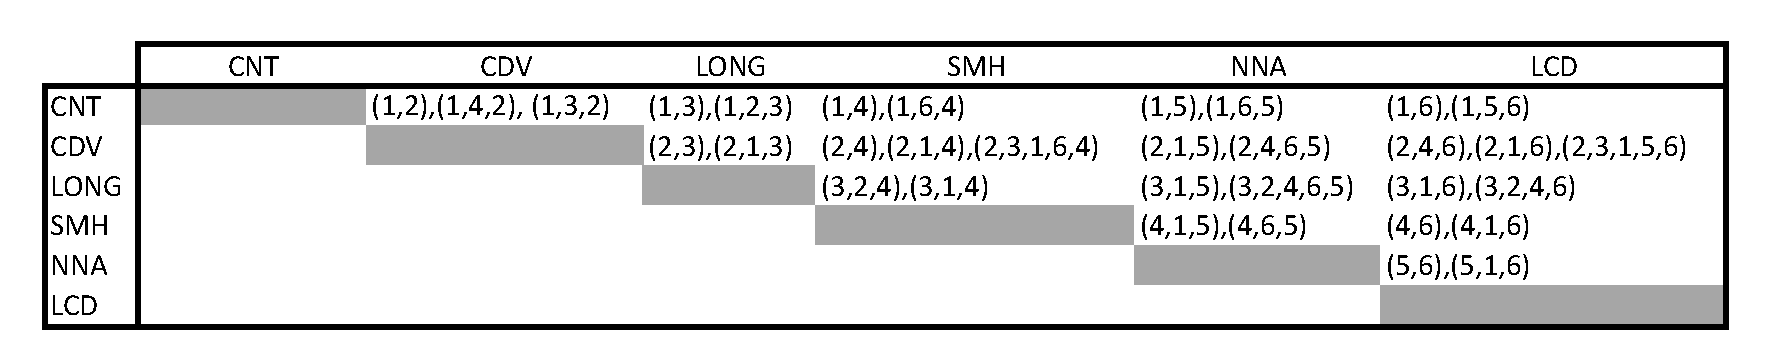
\includegraphics[width=13cm]{Imagenes/caminos}
  \caption[Caminos calculados por algoritmo de disponibilidad]{Caminos que aseguran el estándar de SLA del 0.01\% de indisponibilidad por 2 días. Calculados con algoritmo de la sección \ref{sec:algoritmo_conex}}.
  \label{fig:caminos}
\end{figure}





\begin{itemize}
\item puntos de red a utilizar
\item planos de data centers con distribución de los equipos
\item diagramas de conexión
\item rotulación de fibras, conectores, etc
\item frecuencias
\end{itemize}
